\chapter{Towards a new architecture}
\label{chapter:towards_new_architecture}
The discussion in Chapter \ref{chapter:architecture} concluded with a proposal of a new future-proof architecture. Now, we will shift our focus on efforts on making this design a reality. This will mostly involve building the components that can be found on the higher levels of the proposed architecture, in particular the user interface, the REST API and \emph{libtribler}.

\section{A clear distinction between GUI and core}
As described in Chapter \ref{chapter:problem-description}, the code for the user interface and Tribler core code is interleaved to a large extent and there is no clear separation between these two. There are many instances where we find code present in the user interface code base that should be moved to the core and vice versa. To realise a clear separation between \emph{libtribler} and the user interface, instances like these should be fixed.\\\\
In the current code base, the \emph{Core} package is dependent on the user interface which is a bad situation since this package cannot be reused without shipping the core. The exact dependency is visible in Figure x and is caused by the \emph{DefaultDownloadStartupConfig} class which is located in the \emph{globals.py} file, part of the user interface module. This class is responsible for getting some configuration options in case the user did not override the default options, such as destination of the downloaded file and the amount of anonymous hops used. Since the superclass of \emph{DefaultDownloadStartupConfig}, \emph{DownloadStartupConfig}, is already located in the core, the best option is to move the \emph{DefaultDownloadStartupConfig} class to the \emph{DownloadConfig.py} file, which already contains the \emph{DownloadStartupConfig} class. After we moved this class to the core, the core is completely independent of the user interface.

\begin{figure}[h!]
	\centering
	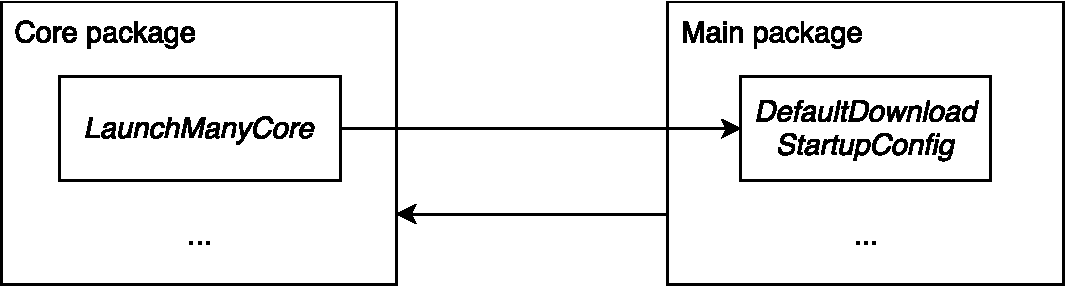
\includegraphics[width=0.6\columnwidth]{images/implementation/cycle_main_core}
	\caption{The cyclic dependency between the core and the main package.}
	\label{fig:cycle-main-core}
\end{figure}

We will now focus on the core package which contains some code that should not be present in the core package. The most interesting piece of interface-related code is attributed to the (embedded) video player in Tribler which is handled by the \emph{VideoPlayer} class in the \emph{Video} package. This class makes use of the VLC bindings for Python, however, the core does not need to have any knowledge about VLC: Managing the video player is a task that should be done on the level of the user interface. Figure \ref{fig:video-package-refactoring-before} shows the \emph{Video} package before refactoring. The \emph{LaunchManyCore} class contains code to start-up all components available in Tribler, including the \emph{VideoPlayer}. This \emph{VideoPlayer} creates a \emph{VideoServer} when being started. Moreover, the \emph{VLCWrapper} class contains various utility methods to work with raw VLC data such as the time position within a video. We removed the \emph{VideoServer} and \emph{VLCWrapper} classes and the composition of the \emph{Video} package after this operation is visible in Figure \ref{fig:video-package-refactoring-after}. We modified the code such that \emph{LaunchManyCore} the starts a video server instead of a video player. We note that there are some classes that appears to be unused, such as \emph{VideoUtility} and \emph{utils}: these classes contains some helper methods to retrieve thumbnail images from a video file. Due to time constraints, we are unable to implement these features in the new user interface so we keep these files as reference for future development.

\begin{figure}
	\centering
	\begin{subfigure}{.5\textwidth}
		\centering
		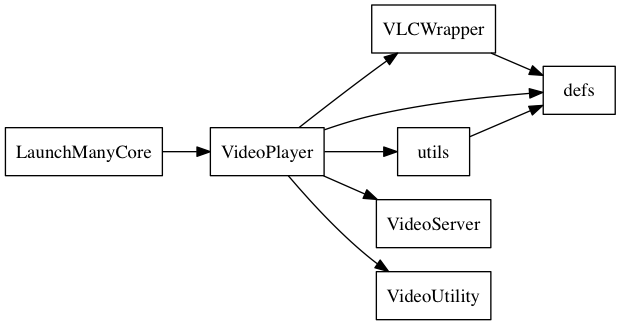
\includegraphics[width=.9\linewidth]{images/implementation/output_video_nov15}
		\caption{Before refactoring}
		\label{fig:video-package-refactoring-before}
	\end{subfigure}%
	\begin{subfigure}{.5\textwidth}
		\centering
		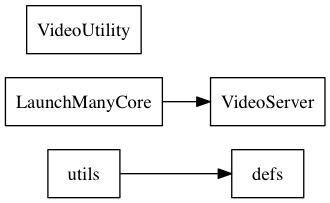
\includegraphics[width=.7\linewidth]{images/implementation/output_video_july16}
		\caption{After refactoring}
		\label{fig:video-package-refactoring-after}
	\end{subfigure}
	\caption{The import graph of the \emph{Video} package in the Tribler core before and after refactoring.}
	\label{fig:video-package-refactoring}
\end{figure}

% link tussen Core -> Main uitleggen

\section{REST API}
As described in Chapter \ref{chapter:architecture}, communication between the graphical user interface and the Tribler core is facilitated using a REST API. This Section explains the implementation of the API in more detail.\\\\
The REST API is written using Twisted. While there are plenty of Python libraries available that allow developers to facilitating a web server in their application, Twisted is used since it already represents a big part of the internal structure of Tribler. With the possibility to integrate the REST API into the main application flow, we avoid having to create special constructions to run the API for instance on a separate thread. API endpoints in Twisted are represented as a resource tree. This is in accordance with REST where the URL of the request can be treated like a path in the resource tree. This structure is also visible to some extent in the import graph of the API module as displayed in Figure \ref{fig:importgraph-api}. We will highlight and discuss some important files in the API module:
\begin{itemize}
	\item \emph{rest\_manager}: the \emph{rest\_manager} file contains the \emph{RESTManager} class which is responsible for starting and stopping the API. In addition, this file contains the \emph{RESTRequest} class which is a subclass of \emph{server.Request} (which in turn is instantiated by Twisted on an incoming request) and handles any exceptions that occurred during the serving of the HTTP request.
	\item \emph{root\_endpoint}: this file hosts the \emph{RootEndpoint} class which represents the root node of our resource tree. This class dispatches incoming requests to the right sub nodes in the tree.
	\item \emph{util}: the \emph{util} file contains various helper functions, such as conversion utilities to easily transform channel and torrent data from the database into JSON format that can be sent to the client that initiated a request.
\end{itemize}

\begin{figure}[h!]
	\centering
	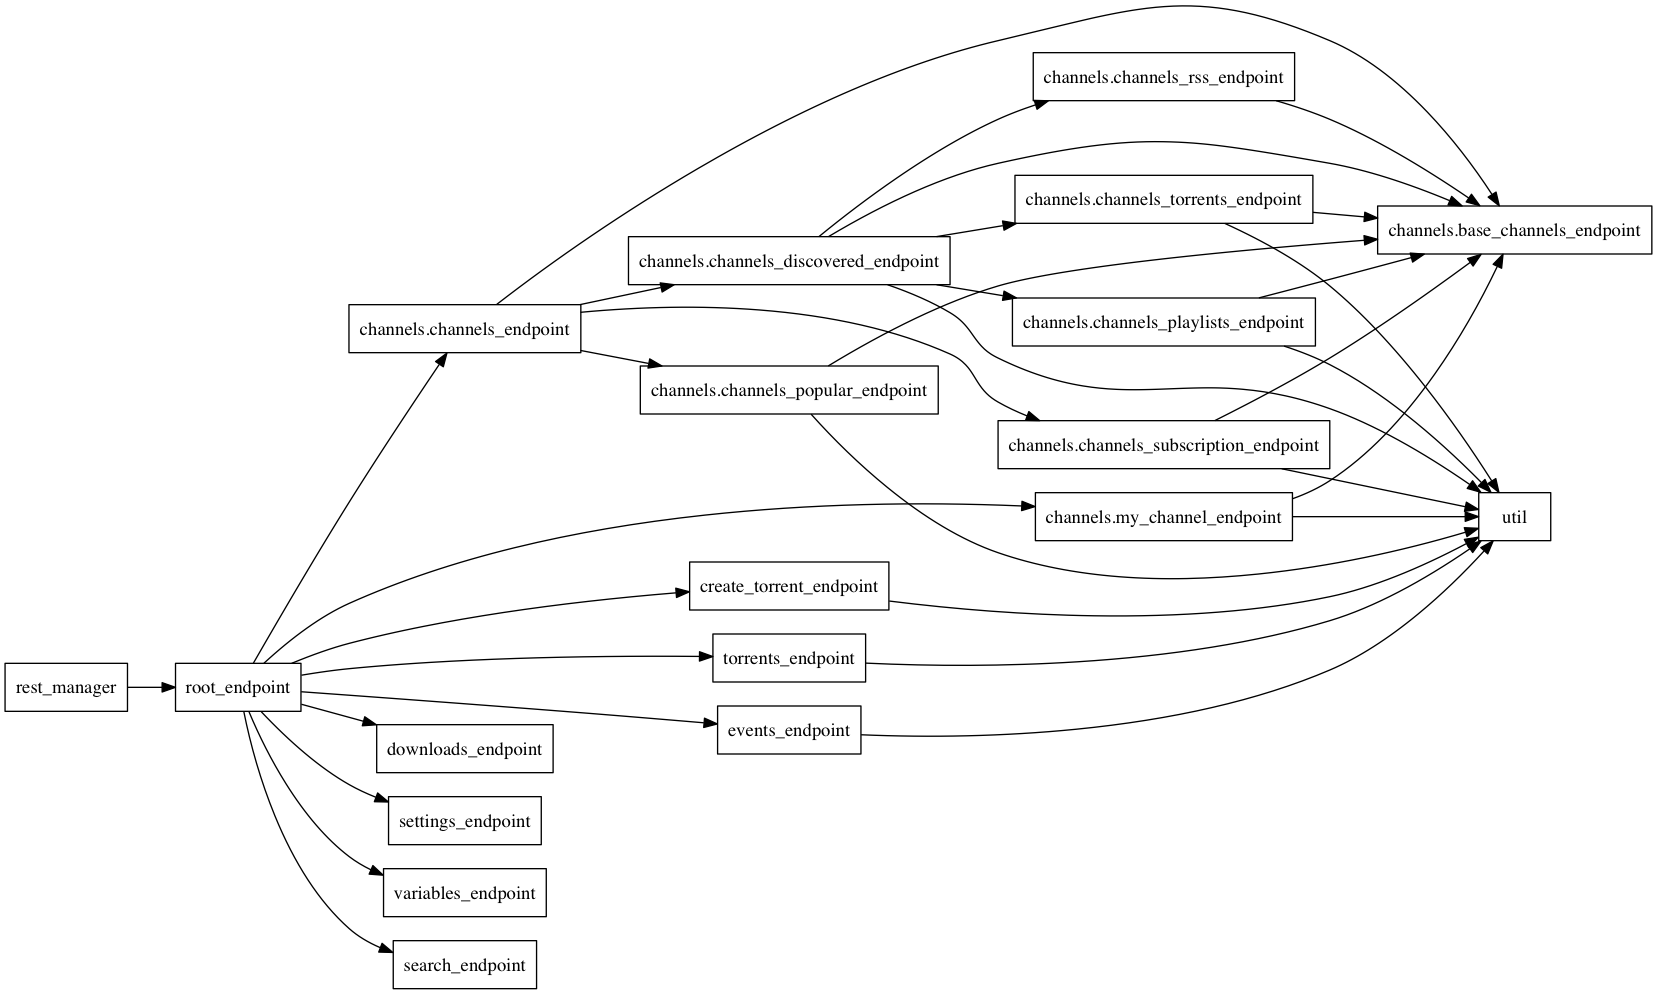
\includegraphics[width=1.0\columnwidth]{images/improving_qa/importgraph_api}
	\caption{The import graph of the REST API module.}
	\label{fig:importgraph-api}
\end{figure}

Except for some endpoints, all data returned by the API is structured in JSON format. The JSON format is well adopted in the field of web engineering and easy to parse. Most of the endpoints are straightforward implementations where the client performs a request and some data is returned. There are situations where the client does a request and a stream of data should be returned. For instance, this is the case when the user performs a search query. Sometimes, data should be returned to the client, even if the client did not ask for this data. When a crash in the Tribler core code occurred, the client should be notified of this crash and possibly warn the user that he or she should restart the application. For this purpose, an asynchronous events stream has been designed and created. Clients can open this event stream and interesting notifications are sent over this stream. All messages that are sent over the \emph{events} connection are shown in Table \ref{table:rest-api-events}.\\

\begin{table}
	\begin{tabularx}{\textwidth}{|l|X|}
		\hline
		\textbf{Event name} & \textbf{Description} \\ \hline
		\emph{events\_start} & The events connection is opened and the server is ready to send events.  \\ \hline
		\emph{search\_result\_channel} & Tribler received a channel search result (either remote or locally). The event contains the channel result data. \\ \hline
		\emph{search\_result\_torrent} & Tribler received a torrent search result (either remote or locally). The event contains the torrent result data. \\ \hline
		\emph{upgrader\_started} & The Tribler upgrader started. \\ \hline
		\emph{upgrader\_tick} & The status of the Tribler upgrader changed. This event contains a human-readable string with the status update. \\ \hline
		\emph{upgrader\_finished} & The Tribler upgrader finished. \\ \hline
		\emph{watch\_folder\_corrupt\_torrent} & The watch folder module has encountered a corrupt .torrent file. The name of the file is part of this emitted event.\\ \hline
		\emph{new\_version\_available} & A new version of Tribler is available. The version number is contained in the event.\\ \hline
		\emph{tribler\_started} & Tribler has completed the startup procedure and is ready to serve HTTP requests on all endpoints.\\ \hline
		\emph{channel\_discovered} & A new channel has been discovered. The events contains the discovered channel data.\\ \hline
		\emph{torrent\_discovered} & A new torrent has been discovered. The events contains the discovered torrent data.\\ \hline
	\end{tabularx}
	\caption{An overview of all events that are passed over the asynchronous events connection, part of the REST API.}
	\label{table:rest-api-events}
\end{table}

The API is started in two stages. Just before starting Tribler, the \emph{events} connection is activated. This connection is initialized earlier so we can send interesting updates of the upgrader to the client. When the upgrader is completed and Tribler has been started, the other endpoints are activated and the API is ready to be used.

\section{Graphical User Interface}
The amount of accumulated technical debt in the current graphical user interface of Tribler is devastating. After going through several development cycles where some impacting changes have been made, the code base of the user interface has reached the point where it is more beneficial to create a complete new user interface. This section will continue the discussion that has been initiated in Section \ref{chapter:problem-description}. First, the structure of the current user interface will be described. Next, the new interface, introduced in Chapter \ref{chapter:architecture} will be elaborated. Encountered design decisions and challenges are presented and discussed.

\subsection{Analysis of the current user interface}
The current user interface is unintuitive and cluttered with widgets and many functionality that should be in the core module of Tribler, can be found at higher levels in the user interface code. There is actually no clear separation between the core and the user interface, making it hard for developers to develop and test new functionalities since they have to deal with a bigger code base. One of the goals of this thesis is to make this separation more explicit for developers so they do not have to touch interface-related code if they are not interested in that.\\\\
The code base of the user interface is full of undesired workarounds and code smells. There is no clear, documented structure to be identified throughout the code and there are several reasons for this issue. One of the underlying causes is the mindset of developers that the user interface code base is subordinate to the code related to the core functionalities of Tribler. While it is often true that minor defects in the user interface are less critical than errors in important core functionalities such as the download engine, developer should always strive to write maintainable code. The fact that the user interface has undergone dramatic changes throughout the 10 years of research is an additional reason that led to this unstructured code base. Making short-term decisions were clearly favoured over decisions that benefit the longer-term development process.\\\\
If we take a closer look at the structure of the user interface code base, several files with many class definitions can be found. In the \emph{widgets.py} file, we can identify 30 distinct widget definitions. The \emph{SearchGridManager} file acts like the glue between the Tribler core and the user interface. Most of the requests to the core are passing through method definitions inside this file.

\subsection{Building a new user interface}
Before starting to create a new user interface, we should first decide which graphical user interface library we would like to use. There are plenty of libraries that are suited for this job. Below, several of such libraries are summarized, together with a small description and some (dis)advantages.
\begin{itemize}
	\item \emph{wxPython}: this is the current user interface library we are using. \emph{wxPython} is built upon \emph{wxWidgets} and provides the Python bindings to this latter library. The library is cross-platform and we can continue to use \emph{wxPython}. We already have a large code base written in \emph{wxPython} so continued usage of this library could allow us to reuse several widgets. The main disadvantages of this library are the minor inconsistencies across different platforms and the lack of a visual designer, requiring us to specify the complete layout in Python code.
	\item \emph{Kivy}: the cross-platform library Kivy has been used by Tribler research, particularly in the past attempts to run Tribler on Android\cite{de2014android}\cite{sabee2014tribler}. The decision of using Kivy for the new user interface enables us to reuse the interface logic on Android. The layout of Kivy can either be created in \emph{.kv} files or specified in code which is based on the separation of concerns principle. While not as old as \emph{wxPython} or \emph{pyQt}, the library has gained significant attention and adoption in the Python community.
	\item \emph{TKinder}: the \emph{TKinder} library is a layer built upon the Tcl/Tk framework and is considered the de-facto graphical user interface library for Python. Like the other discussed frameworks, \emph{TKinder} does not provide a visual designer. The library is built-in in Python which means that no additional libraries have to be installed in order to start writing code. \emph{TKinder} however is considered more suitable for simple applications due to the simplistic nature of the library.
	\item \emph{PyQt}: \emph{PyQt} provides the Python bindings for the Qt framework and is widely used in open-source and commercial applications. With a first version released in 1995, the Qt framework has evolved into a mature state. The library is very well documentation and provides many different addons and plugins to support a wide range of applications. One of these plugins is a visual WYSIWYG designer where the layout of an interface can be specified in a drag-and-drop manner. This generates a \emph{xml} file which can be read and parsed by \emph{Qt}. Visual styles can be specified using the  \emph{Cascading Style Sheet} (CSS) language. The documentation of \emph{Qt} is very comprehensive, although the documentation regarding \emph{PyQt} is somewhat less maintained.
\end{itemize}
Since the graphical user interface will be an important aspect of Tribler, we wish to use a library that is future-proof, well-maintained and easy to use. We think that in the context of this thesis, choosing \emph{PyQt} is the best choice to build a new user interface. The fact that we can specify our layout using an editor is an enormous advantage since this will mean that we have less code to contribute. In addition, this allows other developers that are not familiar with the Tribler code base to contribute to the graphical user interface. The \emph{Qt} visual designer also offers tools for internationalization and translation of the interface in foreign languages. Tasks like these are perfect opportunities for contributions in an open source project and can potentially attract new developers. A screenshot of the used visualizer is visible in Figure x.\\\\
The result of the development of the new interface is displayed in Figure \ref{fig:new-gui-1}. Our vision during development of this interface is that in essence, it should only display data and do as few processing of the data as possible. The majority of the new user interface has been built using the visual designer. Some code has been written to handle requests to the Tribler core, display the right data in lists and to manage interface-related settings. Connections between widgets and Python code are made using the signal-slot mechanism in \emph{Qt}. This mechanism is used for communication between objects and is a central feature in the \emph{Qt} framework. Widgets in \emph{Qt} can have signals, events they want to possibly notify to other widgets. Some widgets have some built-in signals, i.e. a button emits a \emph{clicked} signal if the user clicks the button with the mouse. Other widgets or Python objects can subscribe to these signals. These signals and slots can either be specified using code or the visual designer, however, to keep the amount of Python code to be maintained to a minimum, we decided to specify our widgets connections in the visual designer as much as possible.\\

\begin{figure}[t]
	\centering
	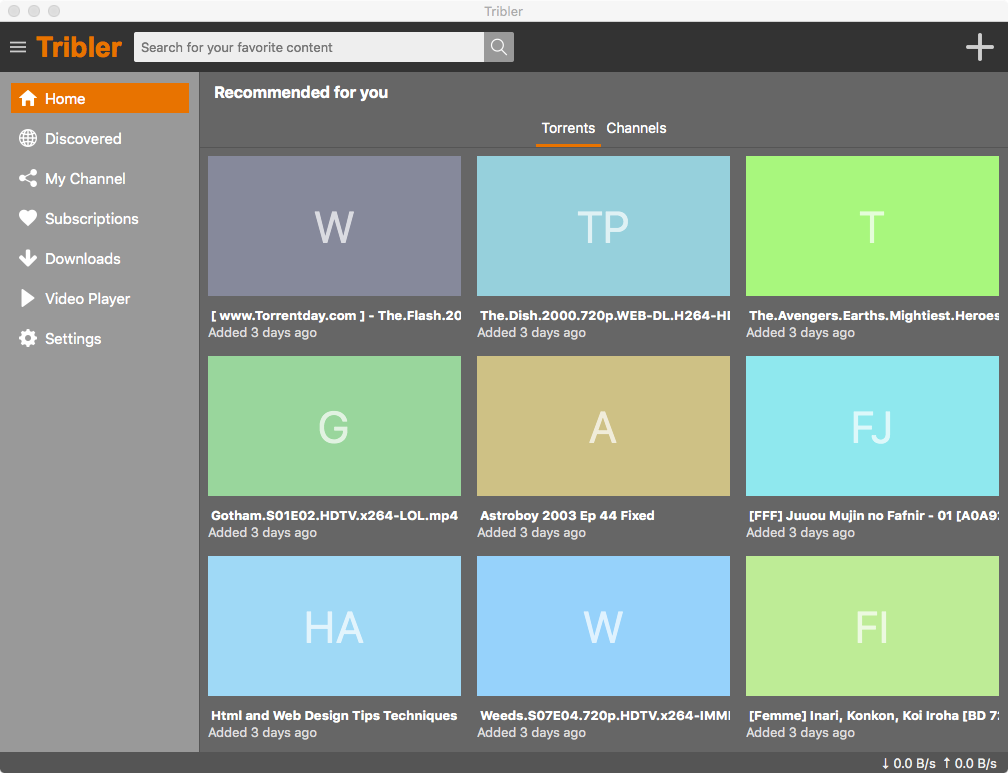
\includegraphics[width=0.8\columnwidth]{images/improving_qa/newgui1}
	\caption{The home page of the new user interface.}
	\label{fig:new-gui-1}
\end{figure}

During development of the user interface, some issues that required some careful analysis were encountered. The remained of the Section will describe these issues in more detail.

\begin{figure}[h!]
	\centering
	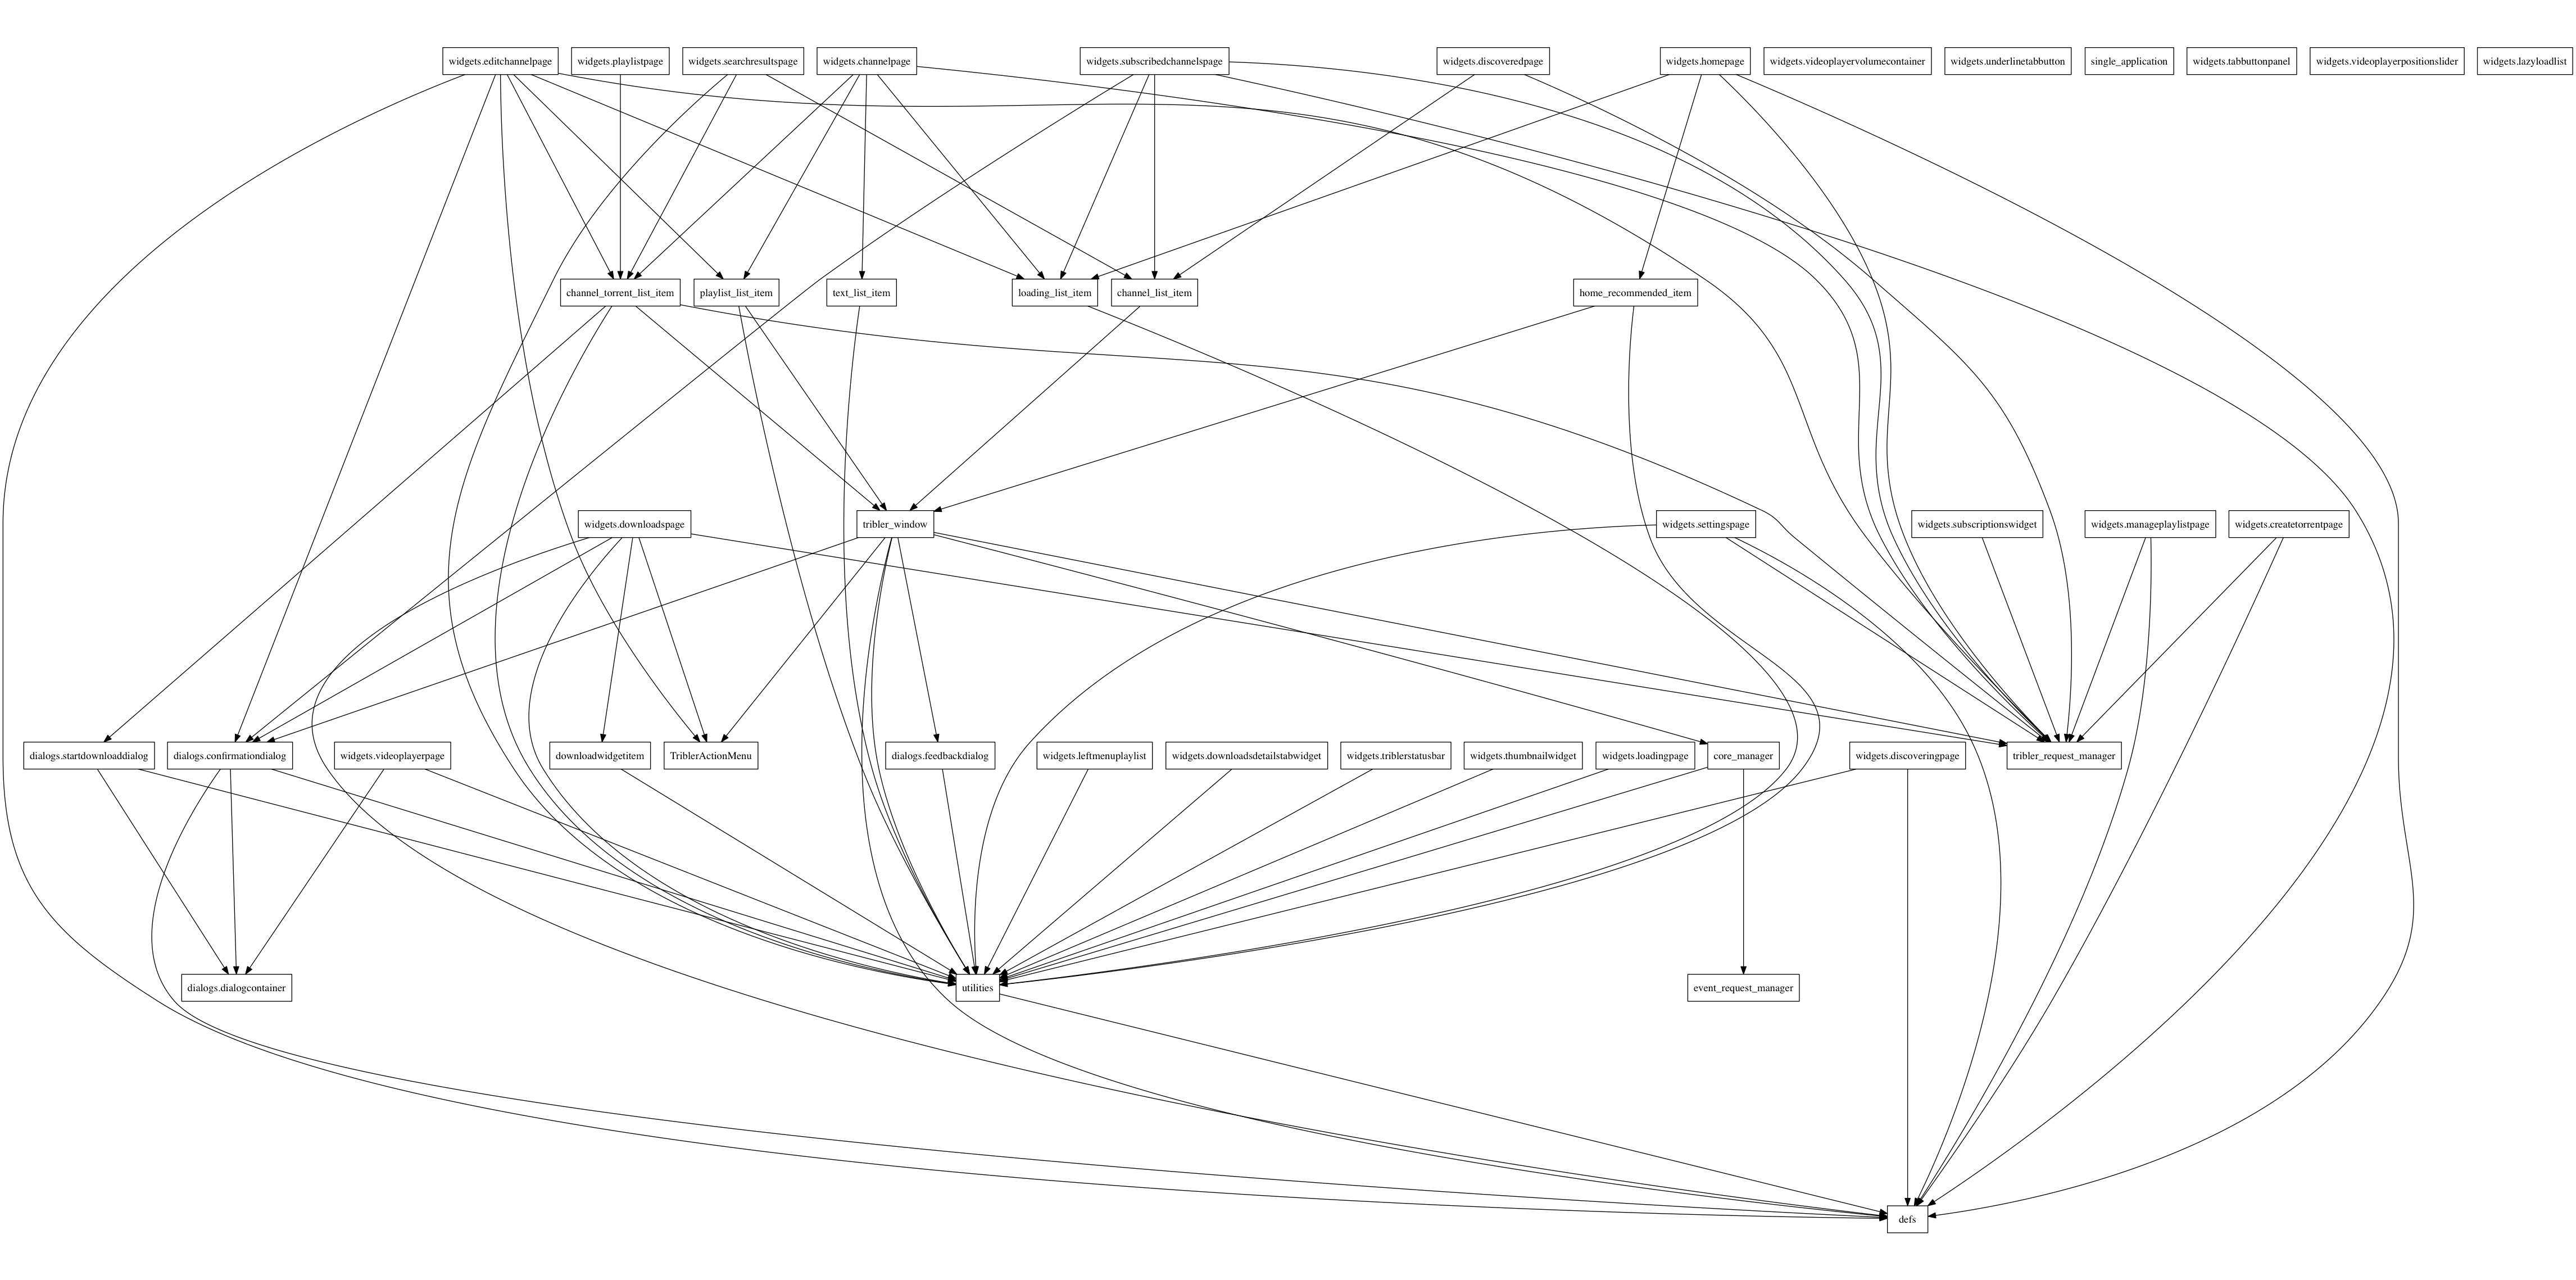
\includegraphics[width=1.0\columnwidth]{images/improving_qa/importgraph_new_gui}
	\caption{The generated import graph of the code base related to the new user interface.}
	\label{fig:importgraph-qt-gui}
\end{figure}

\subsubsection{\textbf{Scalability of list items}}
\emph{Qt} allows to display possibly many items in a simple list. The performance decreases dramatically if custom widgets are rendered in a list, like we are doing. Loading 1.000 of such list items takes over 22 seconds on a high-end iMac device, introducing an unacceptable amount of latency when displaying items. For each item in the list, the associated user interface file has to be loaded, parsed and rendered, possibly many times per second. Channels hold potentially several thousand of torrents which should be displayed in the user interface.\\\\
This problem has been solved by using two techniques. The first one is lazy loading: by using a lazy-loading approach where more data is loaded when the user has scrolled through the end of the list, we can postpone and possibly avoid loading the whole list at once. This solution has also been implemented in the interface written in \emph{wxPython}. By loading only a subset of the list rows, the user experience can be significantly increased since users don't have to wait until the whole list of items is loaded. The implementation of this lazy-loading solution is reusable and can be found in the \emph{lazyloadlist.py} source file. This however, still resulted in a minor period of waiting when the next set of items is being loaded. It turned out that loading the interface definition file every time is a time-consuming operation. The implemented solution to reduce this processing time is to pre-load the interface definition as soon the user interface starts. This has only a minor effect on the total start-up time (around 40 milliseconds on a high-end iMac device).

\subsubsection{\textbf{A working VLC on multiple platform}}
The old user interface made use of the VLC library for the implementation of the embedded video player. This embedded video player did not function on OS X due to incompatibilities with the wx library used. We started the design of the new user interface by creating a prototype where the implementation of a cross-platform, embedded video player with support for starting and stopping a video is centrally involved. While example code was available for the PyQt4 library using VLC bindings, there were some minor quirks when implementing the video player using PyQt5, mostly involved around obtaining a reference to the frame of the video player (which should be done differently for each platform). The code for this player has been used as reference for the implementation of the video player in the new user interface of Tribler and is available on GitHub\cite{vos2016vlc}.

\section{Improvements to the threading model and performance}
The work as described in the last two sections, has led to a better and stable threading model. The complex threading model as used by Tribler 6 is vulnerable for bad code practices, leading to confusion and race conditions.\\\\
Developing the new user interface came with an additional advantage. Now that the user interface runs in a separate process, we have the opportunity to run the reactor on the main thread. This allows us to get rid of the confusing decorators since we only have one thread (besides the threadpool) to schedule calls on. Getting rid of the abundant thread switching should increase performance since we avoid overhead introduced by the context switch. The new threading model is visible in Figure \ref{fig:new-threading-model}.

\begin{figure}[h!]
	\centering
	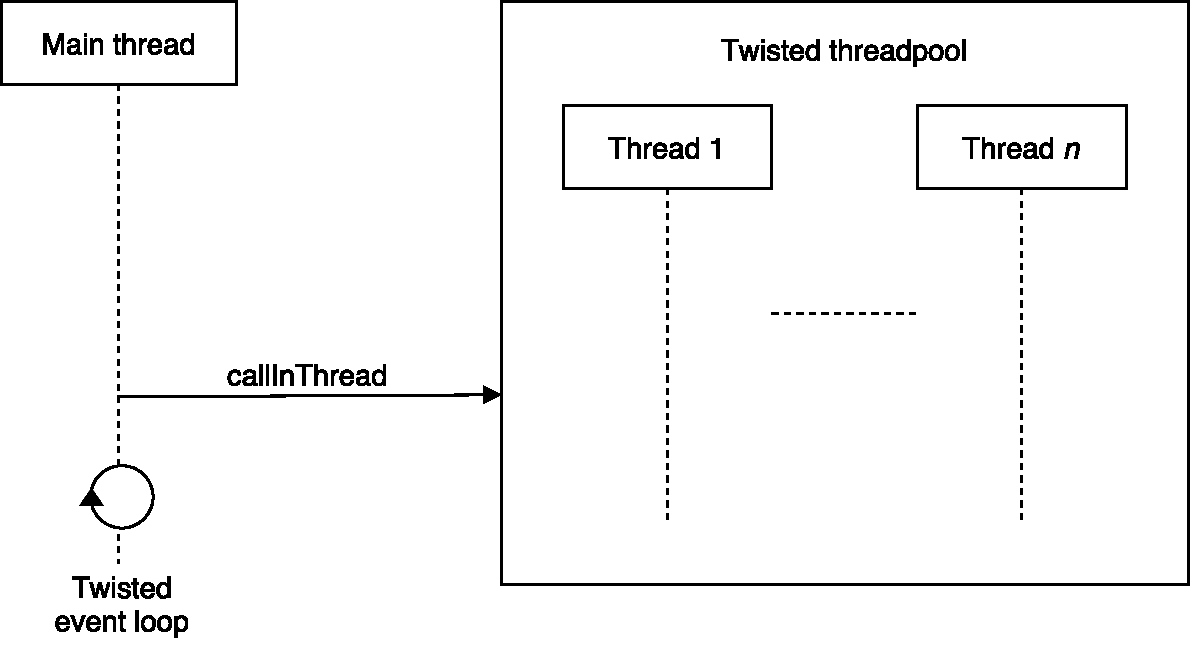
\includegraphics[width=0.7\columnwidth]{images/improving_qa/new_threading_model_tribler}
	\caption{The new, simplified threading model in Tribler 7, together with the primitives to schedule operations on the threadpool.}
	\label{fig:new-threading-model}
\end{figure}

\section{Relevance ranking algorithm}
\label{sec:relevance-ranking-algorithm}
Serving users relevant information as fast as possible is important in Tribler. When users are performing a search in the user interface, the returned search results are sorted according to a relevance ranking algorithm that considers several factors of the search results. A key problem of this algorithm is that the implementation is located inside the code base associated with the user interface. Essentially, sorting search results can be considered a task of the Tribler core. Moving the algorithm to the core module seems to be a adequate solution but this requires us to understand the old relevance ranking rules so we can reimplement the algorithm in the core module. Unfortunately, the code that is responsible for the relevance ranking lacks proper documentation and is hard to read and understand. Moreover, the code it split between several classes, making it harder to understand its behaviour.

\subsection{Old ranking algorithm}
Sorting of channels and torrents are both using a different algorithm. Channels are sorted on the number of torrents where channels that have a higher number of torrents, are displayed higher in the list. The algorithm to sort torrents on relevance is more complex and uses five different scores. These scores are determined as follows (ordered on importance):
\begin{enumerate}
	\item The number of matching keywords in the name of the torrent. Keywords are determined by splitting the name of a torrent on non-alphabetical characters and common keywords such as \emph{the} are filtered out.
	\item The position of the lowest matching keyword in the torrent name. For instance, when searching for \emph{One} and there is a torrent result named \emph{Pioneer-One-S01E03.avi}, the position of the lowest matching keyword is 2, since \emph{Pioneer} is not present in the search query.
	\item The number of matching keywords in the file names that the torrent contains.
	\item The number of matching keywords in the extension of the files (for instance, \emph{avi}, \emph{iso} etc).
	\item A score that is based on several (normalised) attributes of the torrent. This score is determined after the set of local search results are constructed. To calculate this score, the following formula is used: $ s = 0.8 * n_s - 0.1 * n_{vn} + 0.1 * n_{vp} $ where $ s $ is our score, $ n_s $ denotes the number of seeders (0 if this information is not available yet), $ n_{vn} $ the number of negatives votes of this torrent and $ n_{vp} $ the amount of positive votes this torrent has received. We should note that the number of positive and negative votes do not exist any more and as a consequence will always be 0, making this score only dependent on the number of seeders. The normalization process calculates the standard score for every data item, using the following formula:
	
	\begin{equation}
	\label{eq:normalization-standard-score}
	z = \frac{x - \mu}{\sigma}
	\end{equation}
	
	where $ z $ is our normalized score, $ x $ the score to be normalized, $ \mu $ the mean of the data set and $ \sigma $ the standard deviation of the data set.
	
\end{enumerate}
For each torrent, the set of five scores as described above is determined. The comparison between two torrents now proceeds based on these five determined scores, starting with the first score, proceeding to the next score in case when two scores are equal.\\\\
Finally, the list is prepared and a channel result is inserted between every five torrent items in the list. This is done since usually, the amount of torrents is much bigger than the amount of channels. Not only channels matching the search query are displayed: for each torrent, the most popular channel that contains this specific torrent, is determined and also considered in the list of results.\\\\
While the algorithm as described above takes many factors in consideration, we detected some problems and possible improvements:
\begin{itemize}
	\item One of the main problem is that the amount of matches inside a torrent name/torrent file name is not taken into consideration. For instance, when searching for \emph{Pioneer One}, a torrent named \emph{Pioneer One Collection} probably has a higher relevance than a torrent named \emph{Pioneer One - Episode 3, Season 4} since the matching in the first case is considered better.
	\item The relevance sorting of channels in the result set is only dependent on the number of torrents in that channel. The number of matching terms in the channel name and description is not even considered.
	\item When building the inverted index in the SQLite database for the full text search, duplicate words are removed. This means that when we search for \emph{years}, a torrent named \emph{best years} will be ranked equal to a torrent named \emph{years and years} (if we only consider a ranking based on the torrent name). However, the torrent named \emph{years and years} should be assigned a higher relevance since the keyword \emph{years} occurs twice in the latter example. Another example is when searching for \emph{iso}. A torrent file that contains 100 \emph{iso} files is currently ranked equivalent to a torrent file that only has one \emph{iso} file.
	\item The current relevance ranking algorithm only returns results that matches all given keywords. So when searching for \emph{pirate audio}, only torrents are returned that are matching on both terms. It might be better to show the user also torrents matching 'pirate' and matching 'audio' (while still giving a higher relevance score to torrents that matches 'pirate audio').
	\item The ranking of search results are dependent on each other. This is noticeable when calculating the score based on normalized data. To normalize this data, we should have information about other search results. This prevents a "streaming-like" search operation where the relevance score of each search item is only dependent on data that search item contains and no other data.
\end{itemize}

\subsection{Designing a new ranking algorithm}
In the previous Subsection, we described the old ranking algorithm, together with some problems and improvements. In this Subsection, we will design a new, robust and simplified algorithm. The heart of the algorithm will be based on Okapi BM25, a ranking function used by search engines to rank matching documents according to their relevance to a given search query\cite{jones2000probabilistic}. BM25 can be implemented using the following formula:

\begin{equation}
\label{eq:bm25}
s = \sum_{i=1}^{n} IDF(q_i) \frac{f(q_i, D)(k_1 + 1)}{f(q_i, D) + k_1 (1 - b + b * \frac{|D|}{avgdl})}
\end{equation}

In the formula above, we have a document $ D $ where the length of $ D $ is denoted as $ |D| $. There are $ n $ keywords present in our search query, $ q_i $ representing the keyword at index $ i $. $ f(\cdot, D) $ gives the frequency of keyword $ q_i $ in document $ D $. The $ IDF(q_i) $ denotes the \emph{inversed document frequency} of keyword $ q_i $ which basically states how important a keyword is in a document. The IDF is usually calculated as:

\begin{equation}
\label{eq:bm25-idf}
IDF(q_i) = log\frac{N - n(q_i) + 0.5}{n(q_i) + 0.5}
\end{equation}

where $ N $ is the total number of documents and $ n(q_i) $ is the number of documents containing keyword $ q_i $. The full text search engine in SQLite offers tools to easily calculate a BM25 score when performing a query. Unfortunately, this is not implemented in the engine we are currently using, FTS3. This motivates us to upgrade to a newer engine, FTS4, which offers the necessary tools to easily calculate the BM25 score. This requires a one-time upgrade of the database engine of users which should be performed when Tribler starts.\\\\
Each search result is assigned a relevance score. The final relevance score assigned to a torrent is dependent on three other sub-scores that are calculated using the BM25 algorithm and is a weighted average of the sub-scores, determined by the name of the torrent (80\%), the file names of the torrent (10\%) and the file extensions of the torrent (10\%). The final relevance score of a channel is the weighted average of the BM25 score of the name of the channel (80\%) and the description of the channel (20\%).\\\\
While this works well when searching for local search results, we should also be able to assign a relevance rank to incoming remote torrent or channel results. To do this, we keep track of the latest local searches and the gathered information that is used by Equations \ref{eq:bm25} and \ref{eq:bm25-idf}. If we receive an incoming search result, we are using that stored information to quickly determine the relevance score of the remote result. Using this approach, we avoid a lookup in the database for every incoming remote search result. If we have no information about the latest local database lookup available, we assign a relevance score of 0 to the remote result.

\subsection{Ranking in the user interface}
After each search result got a relevance score assigned, we should order the search results in the user interface. We cannot make the assumption that the data we receive from Tribler is already sorted (however, a relevance score should be available) thus we need a way to insert items dynamically in the list. The lazy-loading list we are using in the user interface makes this task more difficult since we both have to insert items dynamically in the list and make sure that we are not rendering too much row widgets. We also wish to avoid reordering operations as they are computational expensive to perform.\\\\
The implemented solution works as follows: in the user interface, we maintain two lists in memory: one list that contains the torrent search results and another list that contains channel search results. We guarantee that these lists are always sorted on relevance score. Insert operations in this list are performed using a binary search to determine the new position of the item in the sorted list, leading to a complexity of $ O(log\ n) $ for each insert operation (where $ n $ is the number of items in the list). In the visible result list, we first display channels, which are usually only a few. The rationale behind this idea is that users prefer to see matching channels since these channels might contain many relevant torrents. This solution is scalable to many search results. The performance of the new relevance ranking algorithm is discussed in Chapter \ref{sec:local-content-search}.